\chapter{A Reinforcement Learning Approach to Black-Box Optimization}

One of the principal challenges in optimization practice is the possibility to optimize in absence of an algebraic model of the system to be optimized. This kind of optimization is known as \textit{black-box optimization}. \\

A black-box function $f(x) : \mathbb{R}^n \rightarrow \mathbb{R}$ is a function for which the analytic form is not known. Nowadays there are lots of mathematical models to succeed in optimize this kind of functions. One of the best known of these methods is the \textit{Bayesian Optimization Model} (BO). \\

In this chapter we will first analyse the state of art of the most used black-box optimization model explaining how BO works and than we will propose an innovative, RL based approach to solve the same problem.

\paragraph{Gaussian Processes} Before introducing BO we have to describe what \textit{Gaussian Processes} (GPs) are. GPs are an alternative approach to regression problems. The GP approach is a \textit{non-parametric} approach (we don't have a priori knowledge of how many parameters will be useful for our regression) to find a distribution over the possible functions $f(x)$ that are consistent with observed data. A GP is a generalization of the Gaussian probability distribution. Whereas a probability distribution describes random variables which are scalars or vectors (for multivariate distributions), a \textit{stochastic process} governs the properties of functions.

GP is a convenient and powerful prior distribution on functions, which we will take here to be of the form 

\begin{equation}
	f : \mathcal{X} \leftarrow \mathbb{R}.
\end{equation}

The GP is defined by the property that any finite set of $N$ points $\{x_n \in \mathcal{X}\}\subsup{}{ n=1}{N}$ induces a multivariate Gaussian distribution  on $\mathbb{R}^N$. The $n$th of these points is taken to be the function value $f(x_n)$~\cite{NIPS2012_4522}. The support and properties of the resulting distribution on functions are determined by a mean function 

\begin{equation}
	m : \mathcal{X} \leftarrow \mathbb{R}
\end{equation}

and by a positive definite covariance function 

\begin{equation}
	k : \mathcal{X} \times \mathcal{X} \leftarrow \mathbb{R}.
\end{equation}

\begin{figure} [h!]
	\centering
	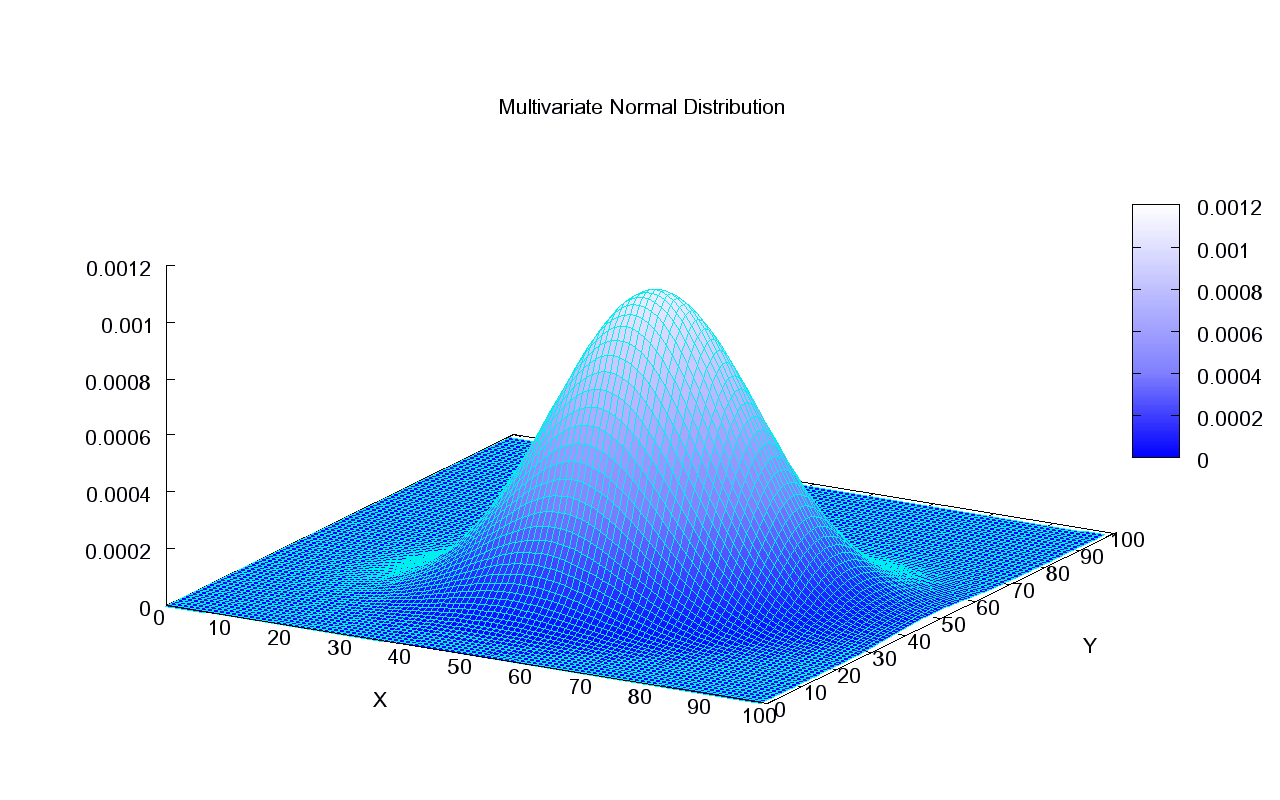
\includegraphics[width= \textwidth, height = 8cm]{Multivariate_Gaussian.png}
	\caption{Multivariate Gaussian Distribution~\cite{MNDWikipedia}}
	\label{fig:Multivatiate_Gaussian}
\end{figure}

\paragraph{Acquisition Functions for Bayesian Optimization} Let's assume that the function $f(x)$ is drawn from a GP prior and that our observation are of the form $\{x_n \in \mathcal{X}\}\subsup{}{ n=1}{N}$, where $y_n \sim \mathcal{N}(f(x_n), v)$ and $v$ is the variance of noise introduced into the function observations. This prior and these data induce  posterior over functions; the acquisition function, which we denote by

\begin{equation}
	a : \mathcal{X} \leftarrow \mathbb{R}^+,
\end{equation}

determines what point in $\mathcal{X}$ should be evaluated next via a proxy optimization

\begin{equation}
	x\textsubscript{next} = \arg\max_{x}a(x),
\end{equation}

where several different functions have been proposed. There are several popular choices of acquisition functions. Under the Gaussian process prior, these functions depend on the model solely through its predictive mean function $\mu(x; \{x_n, y_n\})$ and predictive variance function $\sigma^2(x; \{x_n, y_n\})$~\cite{NIPS2012_4522}.


\begin{figure} [h!]
	\centering
	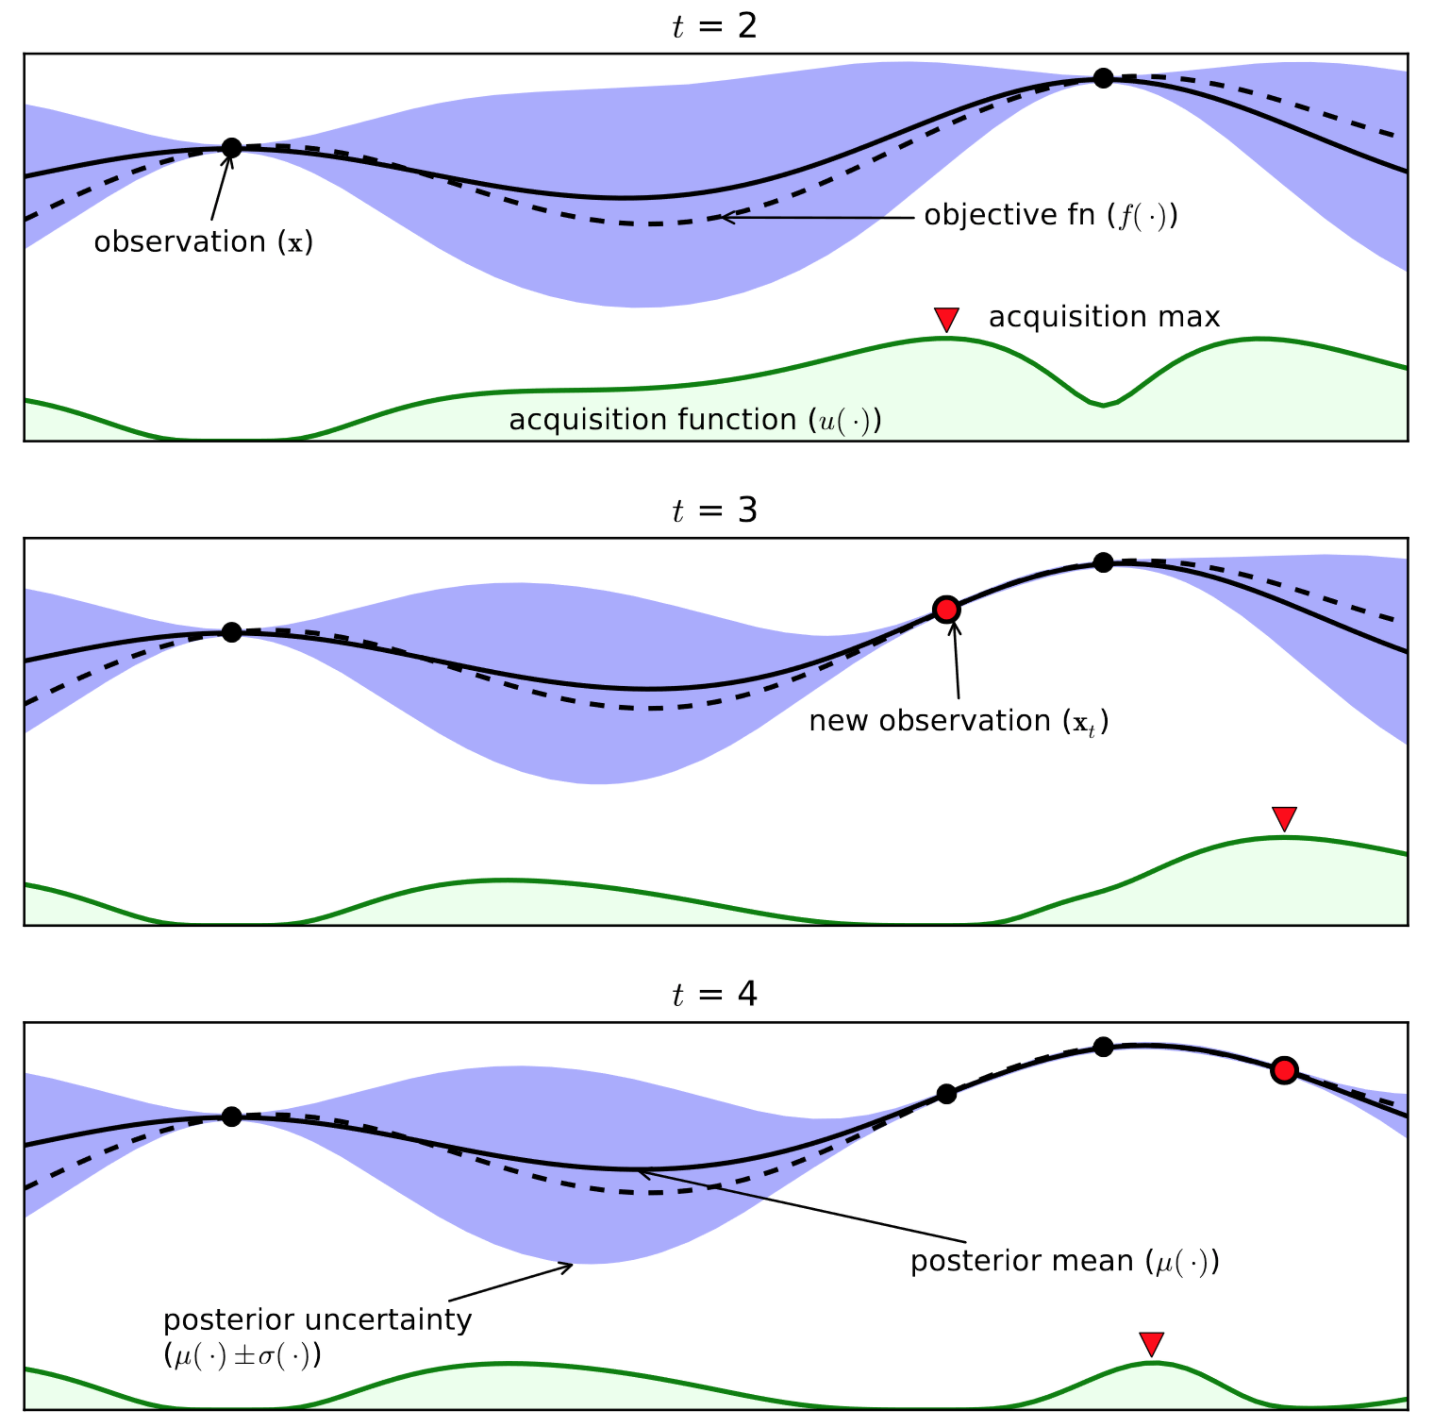
\includegraphics[width= 10cm, height = 10cm]{BOProcess.png}
	\caption{2-$d$ Bayesian Optimization Process Example~\cite{BayesianOptimizationImage}}
	\label{fig:BoProcess}
\end{figure}

\paragraph{An RL Approach To Black-Box Optimization} As previously said, the aim of this thesis is to describe an innovative RL approach to the black-box function optimization problem. Let's assume to dispose of a $3d$-function $f(x, y)$. In this scenario :

\begin{itemize}
	\item \textbf{Agent} : The agent has to maximize a black-box bivariate function. The function is continuously defined over a specific domain. The agent has to complete its job making exactly $150$ epochs for each one of the $1000$ episodes. In each epoch it has a position in space described through the two coordinates $(x, y)$. Each time the agent makes an action the angle between $(x, y)$ and $(x', y')$ and the value of the function $f(x', y')$ are computed.
	\item \textbf{State} : The state is represented by two lists: the first one contains the last two computed \textit{angles} and the second one contains the correspondent last two \textit{actions}.
	\item \textbf{Actions} : In each epoch the agent can make one of four different actions : \textit{move north}, \textit{move  south}, \textit{move east}, \textit{move west}. Each time the agent moves itself of $40$ pixels in one of the previously described directions. The resultant effective movement is computed as follow:
	
	\begin{algorithm} [h!]
		/* knowing $pixelX$ and $pixelY$ */\;
		/* knowing $pixelXRange$ and $pixelYRange$ */ \;
		/* knowing $function$ */\;
		
		\
		
		$domain = function.getDomain()$ \;
		$xRange = domain.maxX - domain.minX$ \;
		$yRange = domain.maxY - domain.minY$ \;
		
		\
		
		$xReal = domain.minX + (pixelX * xRange) / pixelXRange$ \;
		$yReal = domain.minY + (pixelY * yRange) / pixelYRange$ \;
		
		\
		
		\KwRet{$xReal, yReal$}
		\caption{From pixels to real values} 
	\end{algorithm}
	
	\item \textbf{Reward} : In this context we have decided to reward every action of the agent because a real terminal state doesn't exist. Cause we are working with a black-box function we cannot select two coordinate $(x, y)$ and a corresponding value function $z$ as a terminal state. The simulation ends after $1000$ episodes are done. We define a $\Delta$ equals to $\max f(z_n)$ minus $f(z)$ computed in the \textit{current state}:
	
	\begin{equation}
		\Delta = max f(x_n, y_n) - f(x, y)
	\end{equation} 
	
	Our reward at each epoch is equal to $\Delta$.
\end{itemize}

The movement the agent can make in each epoch can be of two different types : \textit{linear movement} or \textit{parametric movement}. If the movement is linear we compute the angle as follow :

\begin{algorithm}
	/* knowing $(x, y)$ */ \;
	/* knowing $(x', y')$*/ \;
	/* {\tt movementAmount} = \textit{M} */ \;
	/* {\tt currentMax} = $\max f(x_n, y_n)$ */ \;
	
	
	\
	
	$z = f(x, y)$ \;
	$z' = f(x', y')$\;
	
	\
	
	$\delta = ((x'-x),  (y'-y))$ \;
	$\alpha = \arctan(\dfrac{\delta}{\tt movementAmount})$
	 
	 \
	 
	 $\Delta = $z'$ - {\tt currentMax} $
	 
	 \caption{Angle computation in linear movement case.} 
	
\end{algorithm}

We can explain this algorithm briefly recalling some trigonometry. Let's suppose to be in a simple 2d case like the one represented in figure ~\ref{fig:LMComputations}.

\begin{figure} [h!]
	\centering
	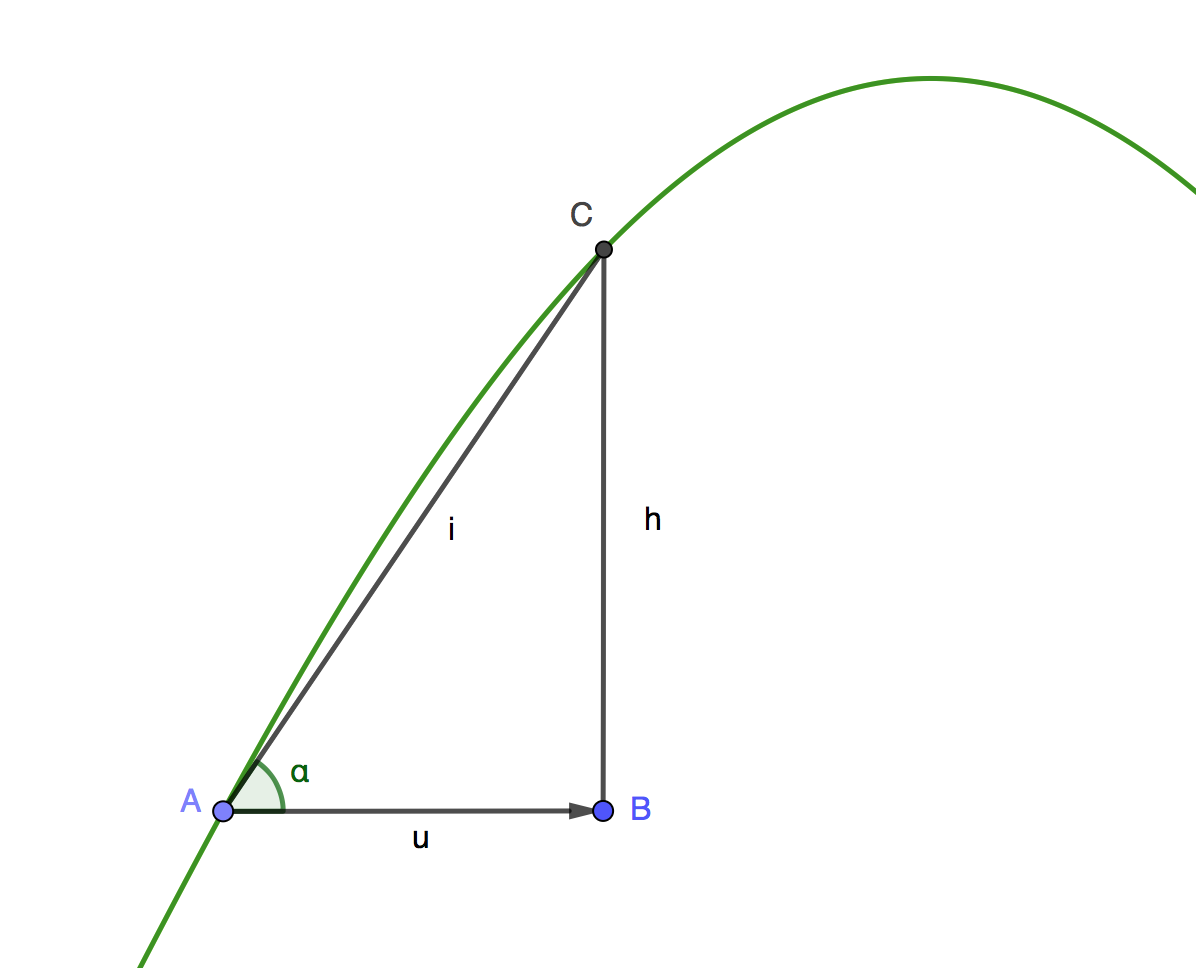
\includegraphics[width= 10cm, height = 9cm]{Triangolo.png}
	\caption{Linear movement computations.}
	\label{fig:LMComputations}
\end{figure}

Let's suppose that the starting point of our RL agent at epoch \textit{e} is the point \textit{A} with coordinates $(x, y)$. In the represented case the agent can make only one of two actions for each epoch : \textit{move on} and \textit{go back}. Making a linear movement of the type \textit{move on} the arriving point at epoch \textit{e'} is \textit{B} with coordinates $(x', y)$. Knowing that the objective function is $f(x) = \sin(2x)$, we can now compute $f(x')$. We now know point \textit{C} with coordinates $(x', f(x'))$. \textit{u} is the {\tt movement amount} and \textit{CB} equals to $f(x') - f(x)$ is $\delta$. From trigonometry we know that 

\begin{equation}
	\tan \alpha = \dfrac{\delta}{\tt movementAmount},
\end{equation}

so 

\begin{equation}
	\alpha = \arctan \dfrac{\delta}{movementAmount}
\end{equation}

If the movement is parametric we want to better approximate the amount of movement over the function. We do this using the following algorithm :

\begin{algorithm}
	/* knowing $(x, y)$ */ \;
	/* knowing $(x', y')$*/ \;
	/* {\tt movementAmount} = \textit{M} */ \;
	/* {\tt currentMax} = $\max f(x_n, y_n)$ */ \;
	
	
	\
	
	$z = f(x, y)$ \;
	$z' = f(x', y')$\;
	
	\
	
	$\delta = ((x'-x),  (y'-y))$ \;
	$\alpha = \arctan(\dfrac{\delta}{\tt movementAmount})$ \;
	
	\
	
	$hypotenuse = \dfrac{{\tt movementAmount}}{\cos \alpha}$ \;
	
	\
	
	$projectionOnHypotenuse = \dfrac{{\tt movementAmount} * {\tt movementAmount}}{hypotenuse}$ \;
	
	\
	
	$realMovementAmount = projectionOnHypotenuse * \cos \alpha$ \;
	 
	 \
	
	$\Delta = $z'$ - {\tt currentMax} $\;
	
	\caption{Angle computation in parametric movement case.} 
	\label{PMAlgo}
	
\end{algorithm}

We can easily explain this algorithm looking at figure ~\ref{fig:PMComputations}. 

\begin{figure} [h!]
	\centering
	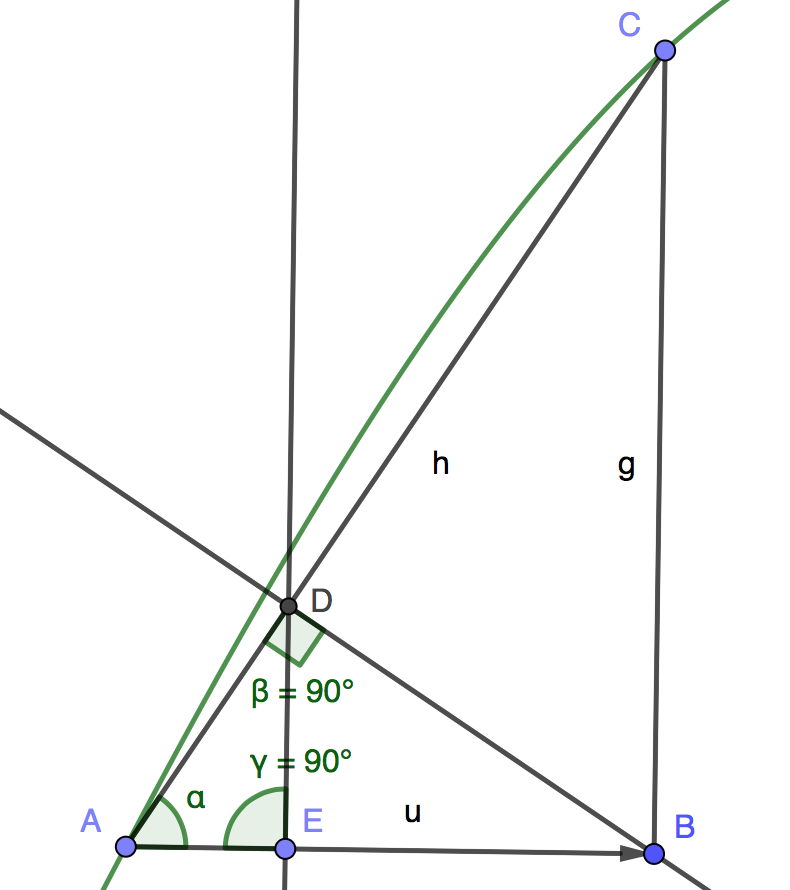
\includegraphics[width= 9cm, height = 9cm]{TRIANGOLO2.png}
	\caption{Parametric movement computations.}
	\label{fig:PMComputations}
\end{figure}

As already previously done, let's suppose that the starting point of our RL agent at epoch \textit{e} is the point \textit{A} with coordinates $(x, y)$. Because of the two dimensions, even in this case the agent can make only one of two actions for each epoch : \textit{move on} and \textit{go back}. Making a linear movement of the type \textit{move on} the arriving point at epoch \textit{e'} is \textit{B} with coordinates $(x', y)$. Knowing that the objective function is $f(x) = \sin(2x)$, we can now compute $f(x')$. We now know point \textit{C} with coordinates $(x', f(x'))$. \textit{u} is the {\tt movement amount} and \textit{CB} equals to $f(x') - f(x)$ is $\delta$. From trigonometry we know $\alpha$ but we are interested in knowing the real amount of movement done by the agent on the function or, at least, its approximation. We want to know how much is $\overline{AB}$.  From the first theorem of Euclid we know that \textit{in a right-angled triangle, the square constructed on a cathetus is equivalent to the rectangle that has for dimensions the hypotenuse and the projection of the cathetus on the hypotenuse}. This means that in a right-angled triangle, the cathetus is proportional medium between the hypotenuse and its own projection on it. According to this we can write the following proportion :

\begin{equation}
	h : u =  u : AD.
\end{equation}

So :

\begin{equation}
	AD = \dfrac{u * u}{h},
\end{equation}

that is the same of :

\begin{equation}
	 pojectionOnHypotenuse = \dfrac{{\tt movementAmount} * {\tt movementAmount}}{hypotenuse}
\end{equation}

of algorithm ~\ref{PMAlgo}. Now we have all elements in order to compute the \textit{real movement amount}. It is simply $\overline{AE}$ segment and it is computed as :

\begin{equation}
	\overline{AE} = \overline{DA} \cos \alpha
\end{equation}

The real question regards why select one method instead of the other one. The answer at this question is simple. Adopting the parametric approach the optimization process is longer but more accurate. In addition to this using the parametric approach we could ideally train our agent on a set of specific functions and it should do very good on a generic function using its knowledge about angles, actions and slope. 

Adopting the linear approach the optimization process is slower but less accurate. In addition to this using the linear approach we couldn't abstract from the concept of function.  This means that for every specific function we have to train our agent one more time.

\subsection{Implementation}

In order to formalize and solve our RL problem, we used the BURLAP (Brown-UMBC Reinforcement Learning and Planning) Java library developed and maintained by James MacGlashan. BURLAP uses a highly flexible system for defining states and and actions of nearly any kind of form, supporting discrete continuous, and relational domains. Planning and learning algorithms range from classic forward search planning to value function-based stochastic planning and learning algorithms~\cite{BURLAPSite}. \\

In order to define specific MDPs, BURLAP offers a set of classes and interfaces (figure ~\ref{fig:UMLBurlap}).

\begin{figure} [h!]
	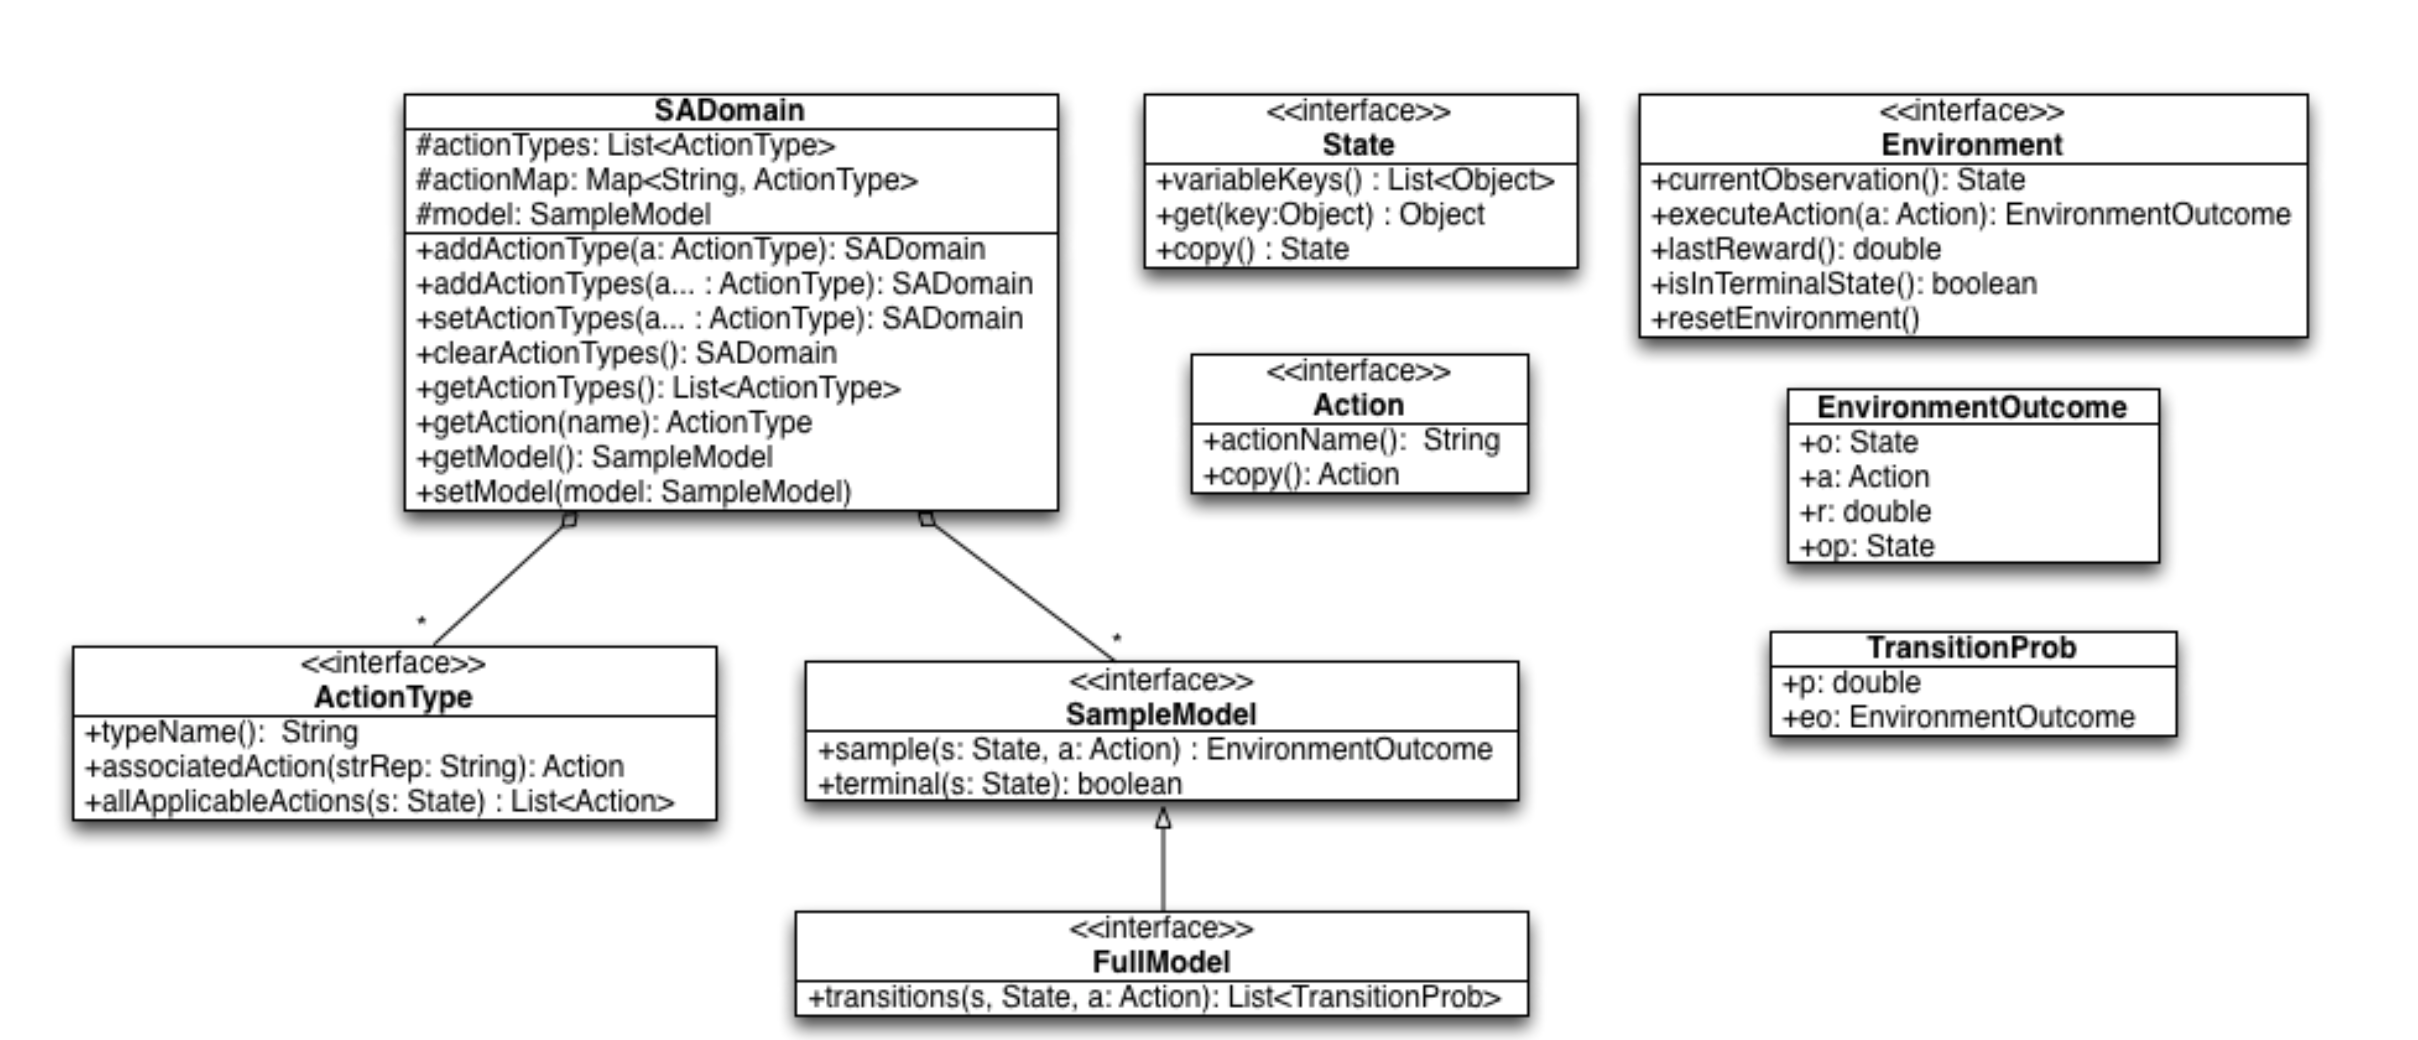
\includegraphics[width= 16cm, height = 9cm]{UMLBurlap.png}
	\caption{UML Digram of the Java interfaces/classes for an MDP definition.}
	\label{fig:UMLBurlap}
\end{figure}

The main features offered by BURLAP are :
	
\begin{itemize}
	\item \textbf{State} : implementing this interface we define the state variables of our MDP state space. An instance of this object will specify a single state from the state space~\cite{BURLAPSite} .
	\item \textbf{Action} : implementing this interface we define a possible action that the agent can select. If our MDP action set is discrete and unparametrized, we may consider using the provided concrete implementation {\tt SimpleAction}, which defines an action entirely by a single string name~\cite{BURLAPSite}.
	\item \textbf{SampleModel} : implementing this interface we define the model of our MDP. This interface only requires us to implement methods that can sample a transition: spit back out a possible next state and reward given a prior state and action taken~\cite{BURLAPSite}.
	\item  \textbf{Environment} : An MDP defines the nature of an environment, but ultimately, an agent will want to interact with an actual environment, either through learning or to execute a policy it computed from planning for the MDP. An environment has a specific state of the world that the agent can only modify by using the MDP actions. Implement this interface to provide an environment with which BURLAP agents can interact. If we define the MDP ourself, then we'll probably don't want to implement {\tt Environment} ourself and instead use the provided concrete {\tt SimulatedEnvironment} class, which takes an {\tt SADomain} with a {\tt SampleModel}, and simulates an environment for it~\cite{BURLAPSite}.
\end{itemize}

An extended definition of classes and interfaces can be found at \url{http://burlap.cs.brown.edu/doc/index.html}.

Starting from features offered by BURLAP, we have extended interfaces and implemented abstract classes in order to modelling the problem described above as shown in figure ~\ref{fig:RLUMLDiagram}. Because of the previous detailed explanation of choices made to model the problem, a deepened analysis of architectural definition is left to the reader.

\begin{figure} [h!]
	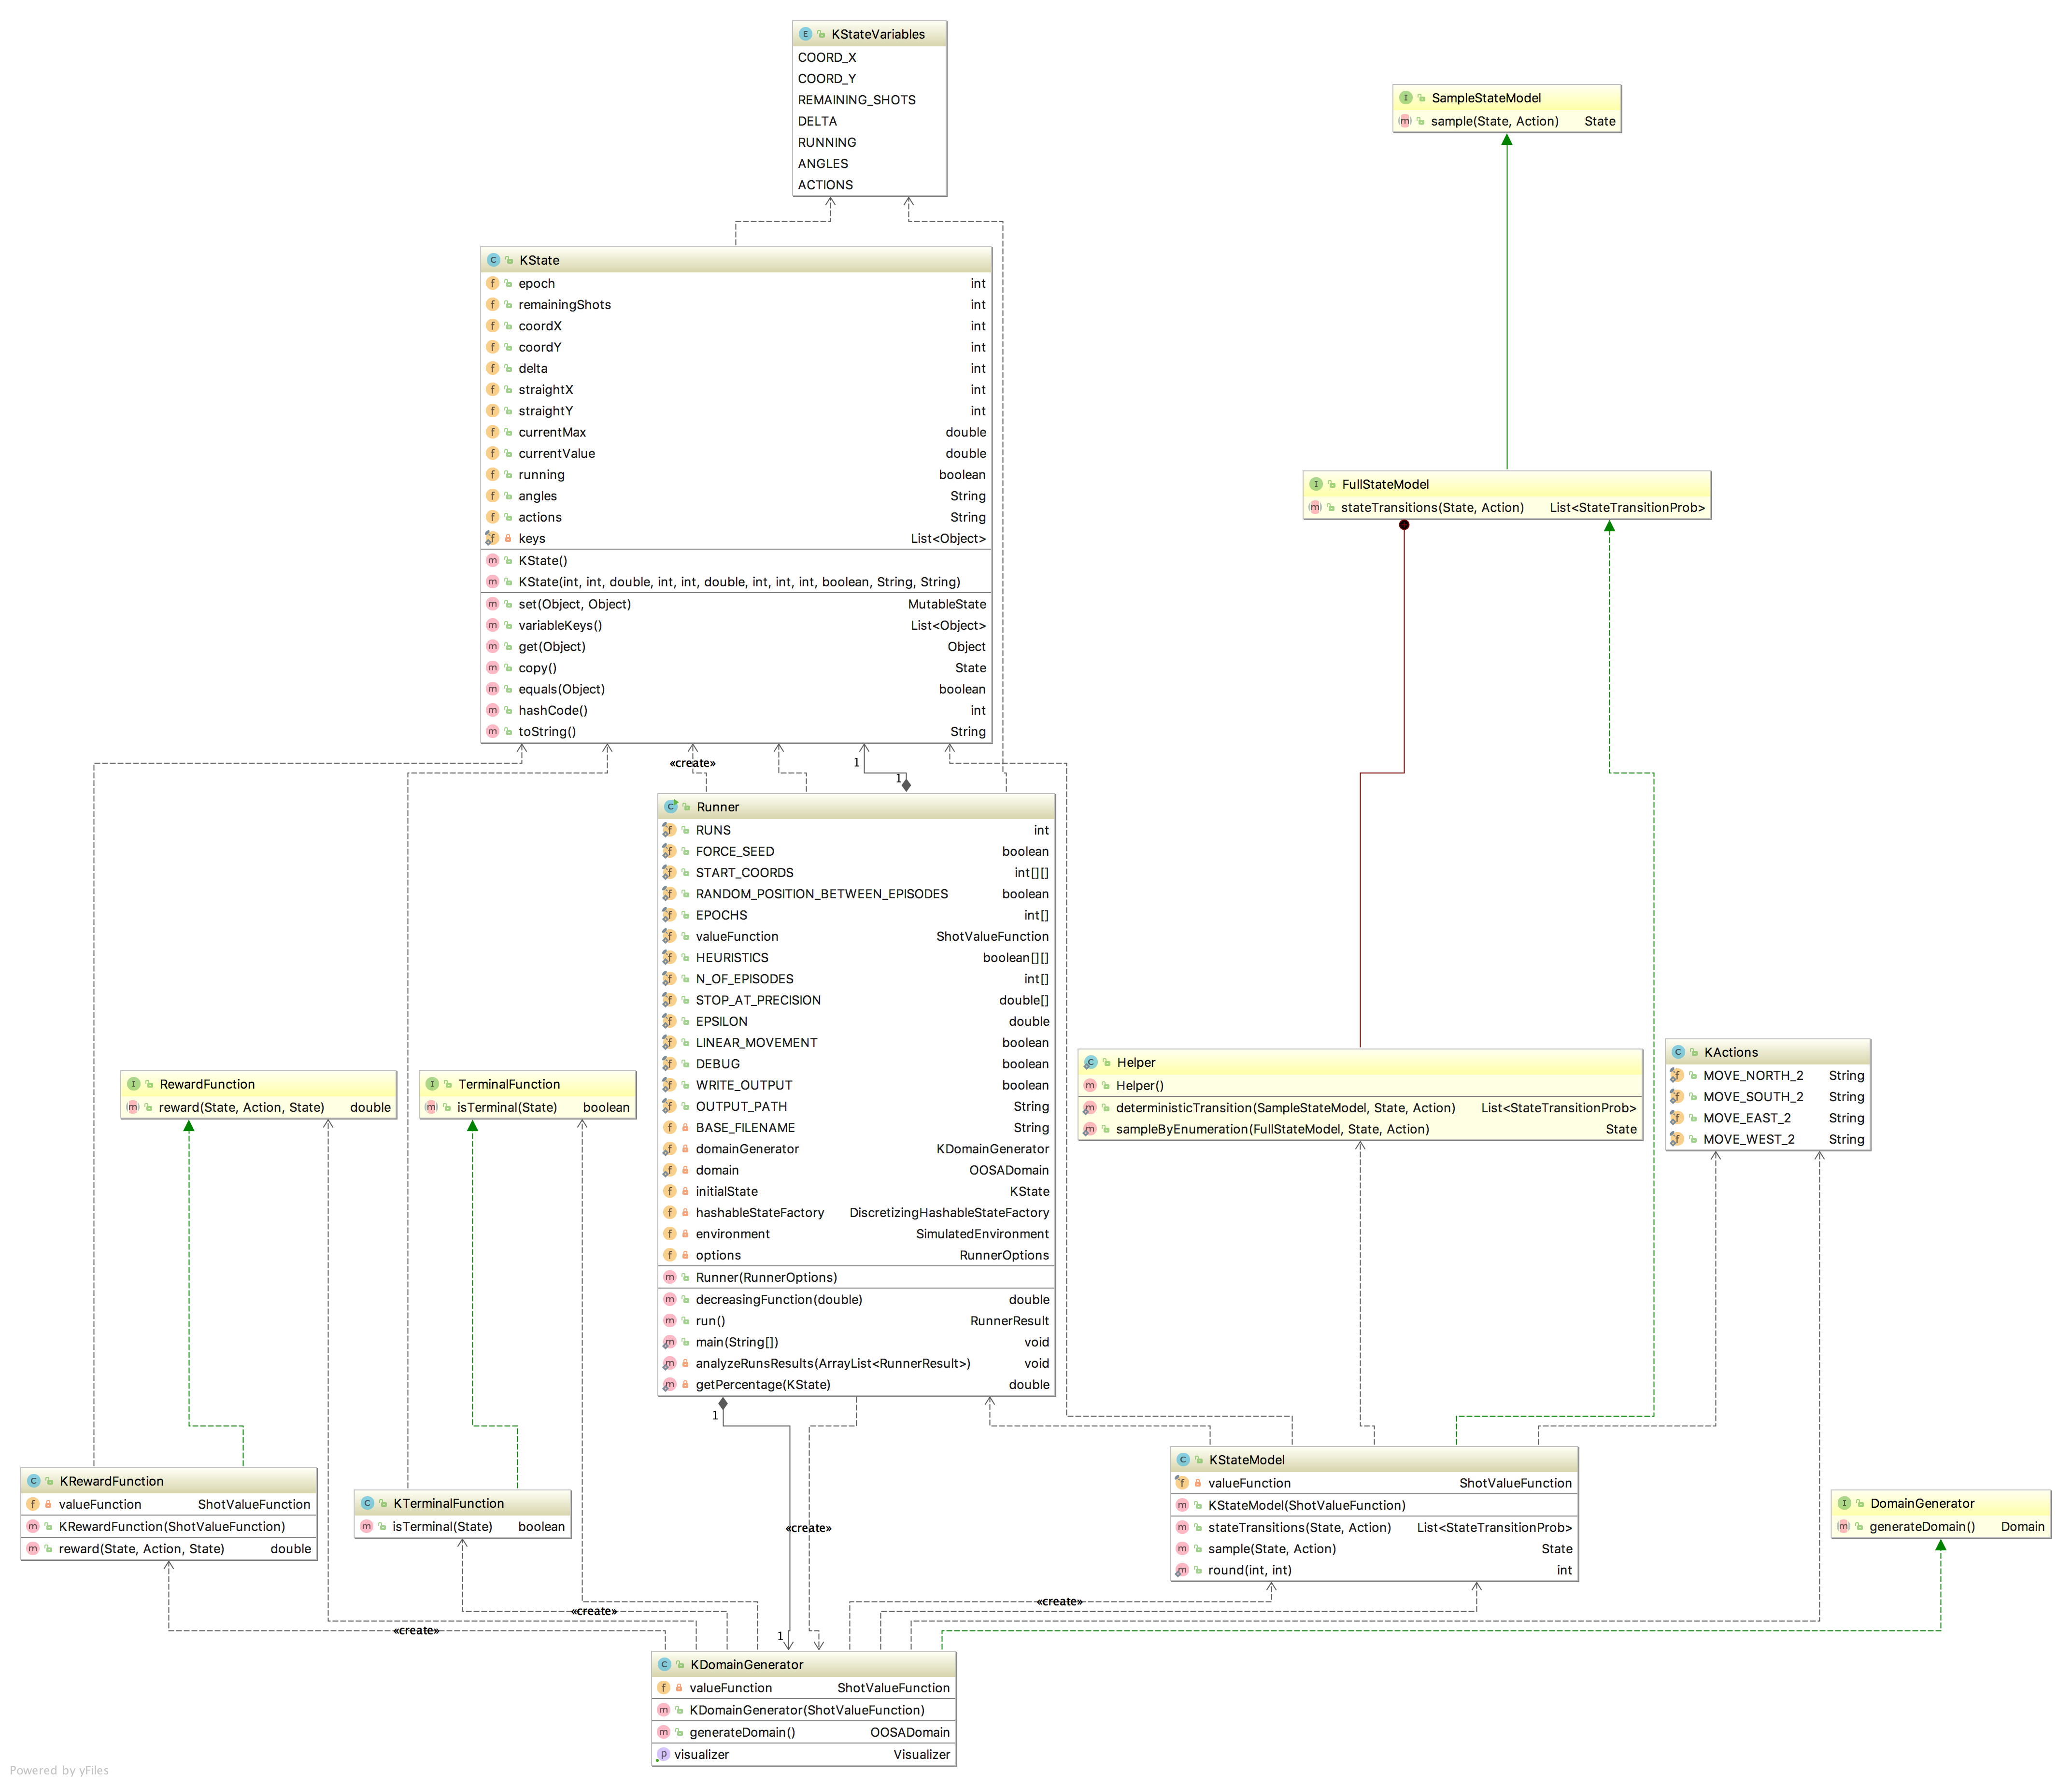
\includegraphics[width= 16cm, height = 18.5cm]{RLDiagram.png}
	\caption{Class diagram of RL black-box optimization tool.}
	\label{fig:RLUMLDiagram}
\end{figure}